% =================================================================
%  学位論文 LaTeX テンプレート
%  コンパイル: latexmk（uplatex + dvipdfmx）  詳細は README.md を参照
% =================================================================

\documentclass[a4j,12pt]{ujreport}

%====[ 論文情報 ]===================================================
% ここを書き換えると，表紙と PDF のメタ情報に反映されます．
\newcommand{\thesisyear}{令和〇年度}                % 年度
\newcommand{\thesistype}{学位論文}                  % 論文種別（卒業論文 / 修士論文 / 博士論文）
\newcommand{\thesistitle}{論文タイトルをここに書く\\（長い場合は改行する）}
\newcommand{\thesistitlepdf}{論文タイトルをここに書く} % PDF用（改行なし）
\newcommand{\thesisadvisor}{指導　教員}              % 指導教員名
\newcommand{\thesisstudentid}{0000 - 0000}          % 学籍番号
\newcommand{\thesisauthor}{氏　名　　太　郎}         % 著者名（表紙用）
\newcommand{\thesisauthorpdf}{Taro Shimei}          % 著者名（PDF用）
\newcommand{\thesisaffiliation}{〇〇大学大学院　〇〇研究科\\〇〇専攻}

%====[ パッケージ ]=================================================
\usepackage[dvipdfmx]{graphicx}
\usepackage{amsmath,amssymb}
\usepackage[dvipdfmx]{xcolor}
\usepackage{url}
\usepackage{fancyhdr}
\usepackage{comment}
\usepackage[nottoc]{tocbibind} % 参考文献・図目次・表目次を目次に載せる
\usepackage[dvipdfmx]{hyperref}
\hypersetup{
  pdftitle  = {\thesistitlepdf},
  pdfauthor = {\thesisauthorpdf},
  bookmarksnumbered = true
}
\usepackage{pxjahyper}
\usepackage[top=30truemm,bottom=30truemm,left=25truemm,right=25truemm,headheight=17pt]{geometry}
\pagestyle{fancy}
\lhead{}
\rhead{\leftmark}
% ヘッダを「第1章 序論」の形式にする
\renewcommand{\chaptermark}[1]{\markboth{\ifnum\value{chapter}>0 \prechaptername\thechapter\postchaptername\quad\fi #1}{}}

% !TEX root = 00_main.tex
% =================================================================
%  マクロ定義
% =================================================================

% 図表・章・式の参照
%   ラベルは \label{fig:xxx} \label{tab:xxx} \label{chap:xxx} \label{eq:xxx} の形で付ける．
%   本文中では \figref{xxx} → 「図 1.1」のように出力される．
\newcommand\figref[1]{図~\ref{fig:#1}}
\newcommand\tabref[1]{表~\ref{tab:#1}}
\newcommand\chapref[1]{第~\ref{chap:#1}~章}
\newcommand\secref[1]{\ref{sec:#1}~節}
\newcommand\equref[1]{式~(\ref{eq:#1})}

\renewcommand{\bibname}{参考文献}

% 行間
\def\baselinestretch{1.15} \small\normalsize

% 執筆中のメモ（赤字で表示）
%   \todo{あとで図を追加} のように使う．
%   提出前に下の \showtodotrue を \showtodofalse にすると全て非表示になる．
\newif\ifshowtodo
\showtodotrue
\newcommand{\todo}[1]{\ifshowtodo\textcolor{red}{\textbf{[TODO: #1]}}\fi}


\begin{document}

%====[ 表紙 ]========================================================
\pagenumbering{alph} % 本文のページ番号と PDF 内部で衝突しないようにする
% !TEX root = 00_main.tex
% 表紙．内容は 00_main.tex の「論文情報」で設定する．
\begin{titlepage}
  \begin{center}
    \vspace*{2zh}
    {\LARGE\bf \thesisyear\thesistype}\\
    \vspace*{6zh}
    {\LARGE\bf \thesistitle}\\
    \vspace*{8zh}
    {\Large\bf 指導教員}\\
    \vspace*{1zh}
    {\Large \thesisadvisor}\\
    \vspace*{4zh}
    {\Large\bf 学籍番号}\\
    \vspace*{1zh}
    {\Large \thesisstudentid}\\
    \vspace*{3zh}
    {\Large\bf \thesisauthor}\\
    \vspace*{6zh}
    {\large \thesisaffiliation}\\
  \end{center}
\end{titlepage}


%====[ 概要 ]========================================================
\pagenumbering{roman}
% !TEX root = 00_main.tex
\chapter*{概要}
\markboth{概要}{}
% 背景，課題，目的，作ったもの，実験，結果を簡潔に書く（目安：1ページ以内）

% 背景・課題
ここに研究の背景と課題を書く．

% 目的・提案
ここに研究の目的と，提案する手法・システムの概要を書く．

% 実験
ここに実施した実験・評価の概要を書く．

% 結果
ここに得られた結果と，そこから言えることを書く．

\pagebreak


%====[ 目次 ]========================================================
\tableofcontents
\markboth{\contentsname}{}
\pagebreak

%====[ 本文 ]========================================================
% 章を増減する場合はファイルを追加・削除して，ここの \input を編集する．
\pagenumbering{arabic}
% !TEX root = 00_main.tex
\chapter{序論}\label{chap:introduction}

\section{背景}\label{sec:background}
% 社会的背景 → 現状の問題 → 解決すべき課題 の順に書く．
% 主張には必ず根拠（参考文献）を付ける．例：\cite{sample-book}
ここに研究の背景を書く．
\todo{ここに統計データを追加する}
文献を引用する場合は\verb|\cite{キー}|を用いる\cite{sample-book}\cite{sample-web}．
書きかけの箇所には\verb|\todo{...}|でメモを残せる（提出前に\verb|01_macro.tex|の設定で一括非表示にできる）．

\section{目的}\label{sec:purpose}
% 本研究で何を明らかにする／何を作るのかを明確に書く．
ここに研究の目的を書く．

\section{本論文の構成}
本論文の構成は以下の通りである．
\chapref{related-work}では関連研究について述べ，本研究の位置づけを示す．
\chapref{method}では提案手法について述べる．
\chapref{implementation}では提案手法の実装について述べる．
\chapref{evaluation}では評価実験とその結果について述べる．
最後に\chapref{conclusion}で結論を述べる．

% !TEX root = 00_main.tex
\chapter{関連研究}\label{chap:related-work}
本章では，本研究に関連する研究について述べる．

\section{〇〇に関する研究}
% 先行研究を紹介し，それぞれの特徴と限界を述べる．
ここに関連研究を書く\cite{sample-article}\cite{sample-proceedings}．

\section{本研究の位置づけ}
% 先行研究で解決されていない点と，本研究のアプローチを述べる．
ここに本研究の位置づけを書く．

% !TEX root = 00_main.tex
\chapter{提案手法}\label{chap:method}
本章では，提案手法について述べる．
以下に，論文でよく使う記法の例を示す（不要になったら削除してよい）．

\section{図の挿入例}
図は\verb|graphics/|ディレクトリに PDF 形式で置き，\figref{sample}のように参照する．

\begin{figure}[htb]
  \centering
  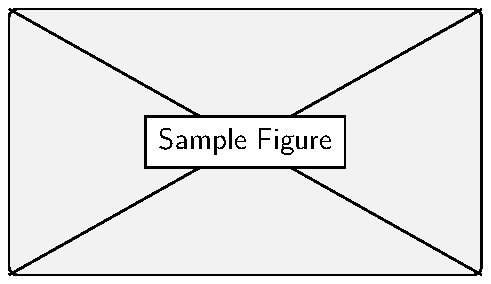
\includegraphics[width=0.6\textwidth]{graphics/sample.pdf}
  \caption{サンプル図}
  \label{fig:sample}
\end{figure}

\section{表の挿入例}
表は\tabref{sample}のように参照する．
表のキャプションは表の上に，図のキャプションは図の下に置くのが一般的である．

\begin{table}[htb]
  \centering
  \caption{サンプル表}
  \label{tab:sample}
  \begin{tabular}{|l|c|c|} \hline
    手法     & 精度 [\%] & 処理時間 [s] \\ \hline \hline
    従来手法 & 80.0      & 1.2          \\ \hline
    提案手法 & 90.0      & 0.8          \\ \hline
  \end{tabular}
\end{table}

\section{数式の例}
番号付きの数式は\equref{sample}のように参照する．
\begin{equation}
  E = \frac{1}{N} \sum_{i=1}^{N} (y_i - \hat{y}_i)^2
  \label{eq:sample}
\end{equation}
文中の数式は $x^2 + y^2 = r^2$ のように書く．

\section{箇条書きの例}
\begin{itemize}
  \item 項目1
  \item 項目2
\end{itemize}

\begin{enumerate}
  \item 手順1
  \item 手順2
\end{enumerate}

\section{コメントアウト}
% 1行だけなら % を使う．
\begin{comment}
  複数行をまとめて PDF に出力しないようにするには
  comment 環境を使う．
\end{comment}
メモや下書きは\verb|%|や\verb|comment|環境で残しておくとよい．

% !TEX root = 00_main.tex
\chapter{実装}\label{chap:implementation}
本章では，\chapref{method}で述べた提案手法の実装について述べる．

\section{システム構成}
ここにシステム構成を書く．

\section{実装環境}
ここに実装環境（言語，ライブラリ，ハードウェアなど）を書く．

% !TEX root = 00_main.tex
\chapter{評価実験}\label{chap:evaluation}
本章では，提案手法の評価実験について述べる．

\section{実験概要}
% 目的，実験環境，対象者（参加者），手続きを再現できるように書く．
\subsection{目的}
ここに実験の目的を書く．

\subsection{実験環境}
ここに実験環境を書く．

\subsection{対象者}
ここに対象者を書く．

\subsection{手続き}
ここに実験の手続きを書く．

\section{結果}
% 事実（データ）のみを書く．解釈は考察で書く．
ここに実験結果を書く．

\section{考察}
ここに結果の考察を書く．

% !TEX root = 00_main.tex
\chapter{結論}\label{chap:conclusion}

\section{まとめ}
% 目的に対して何をして，何がわかったのかをまとめる．
ここに本研究のまとめを書く．

\section{今後の課題}
ここに今後の課題と展望を書く．

\clearpage


%====[ 謝辞 ]========================================================
% !TEX root = 00_main.tex
\chapter*{謝辞}
\addcontentsline{toc}{chapter}{謝辞}
\markboth{謝辞}{}
% 謝辞は「です・ます」調で書くため，文体チェックを無効にする
% textlint-disable ja-technical-writing/no-mix-dearu-desumasu
本研究を進めるにあたり，ご指導を賜りました〇〇大学 〇〇教授に心から感謝いたします．

ここに謝辞を書く．
% textlint-enable ja-technical-writing/no-mix-dearu-desumasu

\clearpage


%====[ 参考文献 ]====================================================
% !TEX root = 00_main.tex
% 参考文献
%   文献情報は references.bib に BibTeX 形式で書き，本文中で \cite{キー} と引用する．
%   引用した文献だけがリストに出力される．
%   スタイル: junsrt（引用順・日本語対応）．著者名順にしたい場合は jplain にする．
\bibliographystyle{junsrt}
\bibliography{references}


%====[ 図・表一覧 ]==================================================
% !TEX root = 00_main.tex
% 図目次・表目次（目次への登録は tocbibind パッケージが行う）
\listoffigures
\clearpage

\listoftables
\clearpage


%====[ 研究業績 ]====================================================
% !TEX root = 00_main.tex
\chapter*{本学位論文に関する著者の発表論文リスト}
\addcontentsline{toc}{chapter}{本学位論文に関する著者の発表論文リスト}
\markboth{発表論文リスト}{}
\begin{enumerate}
\item 著者1, 著者2, 著者3: "発表タイトル", 学会名, (2020.06).
\item Author, A., \& Author, B. (2020, March). Title of the paper. In Conference Name.
\end{enumerate}


%====[ 付録 ]========================================================
% !TEX root = 00_main.tex
\chapter*{付録}
\addcontentsline{toc}{chapter}{付録}
\appendix
\markboth{付録}{}

% アンケート用紙などの PDF を載せる例（page= でページを指定）
% \begin{center}
%   \includegraphics[page=1,width=0.85\textwidth]{graphics/questionnaire.pdf}
% \end{center}
ここに付録を書く．


\end{document}
